\chapter{La herramientas del inversor}

\section{Tipos de gráficos}


Veremos los diferentes tipos de gráficos que se utilizan en las plataformas de \ti{trading}. 

\begin{enumerate}
    \item \tb{Gráficos de línea}, lo que se visualiza es una línea contínua que une los diferentes precios de cierre para diferentes períodos. La información que presentan es muy escasa, si bien puede ser útil en cierto momentos para visualizar claramente  en qué puntos se han detenido esos precios y puede existir un cambio de tendencia.
    \begin{center}
        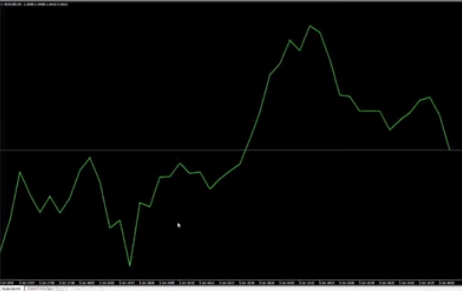
\includegraphics[scale=.95]{images/graphs-01.png}
    \end{center}
    En el gráfico vemos que se han unido precios de cierre en diferentes momentos del tiempo. Es una línea continua, sin más información, donde a veces se puede parar la cotización y continúa luego un cambio de tendencia; esa línea se va formando y es variable hasta que la línea no quede fija.
    \item \tb{Gráficos de barras}, aporta mucha más información que el anterior; tenemos por un lado una barra vertical que nos informa del máximo y del mínimo de precio cotizado en un período de tiempo determinado, si hablamos de datos diarios sería el máximo cotizado en el día, y como mínimo el precio más bajo cotizado. También aporta información, una barra lateral izquierda, de la apertura o primer precio cotizado y hacia la derecha otra línea que nos informa del precio de cierre en ese período de tiempo último cotizado.
    \begin{center}
        \begin{tabular}{ c c }
            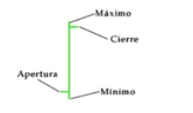
\includegraphics[scale=.65]{images/graphs-02_01.png} &
            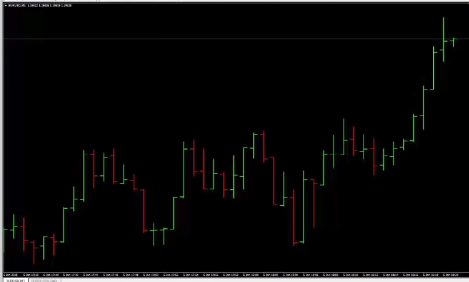
\includegraphics[scale=.65]{images/graphs-02.png}
        \end{tabular}
    \end{center}
    Normalmente, las plataformas de \ti{trading} suelen configurar con color \ti{verde} aquellas en las que el precio de apertura es más bajo que el precio de cierre, indica que a subido el precio en ese período de tiempo, y en \ti{rojo} cuando el precio de apertura es más alto que el de cierre. 
    Vemos en el gráfico que la última barra se está formando poco a poco en ese período de tiempo y no finaliza, la barra derecha no se completa, hasta que se produzca el cierre, durante ese tiempo oscilará hacia arriba o hacia abajo hasta que finalice el período de tiempo. Una vez finalizado quedará formada dicha barra derecha, en color \ti{verde} o en \ti{rojo} según el caso.
    \item \tb{Gráficos de velas japonesas o candlestick}, la información nos facilita es parecida o similar a la de los gráficos de barras, un máximo y mínimo de apertura y cierre, en este caso vemos que la barra tiene un cuerpo y unas mechas, en este caso si la apertura y el cierre van de \ti{menos a más} o de \ti{más a menos} cambiará el color:
    \begin{itemize}
        \item \ti{blanco} para las velas \ti{alcistas de apertura más baja que el cierre}.
        \item \ti{negra} para aquellas en que el \ti{cierre es más bajo que la apertura}.
    \end{itemize}
    Los colores pueden configurarse, como en el siguiente gráfico, donde las \ti{velas alcistas son de color verde}, mientras que las \ti{bajistas son rojas}.
    \begin{center}
        \begin{tabular}{ c c }
            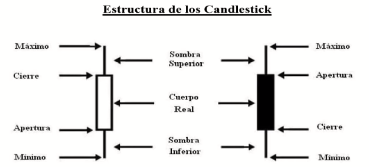
\includegraphics[scale=.65]{images/graphs-03_01.png} &
            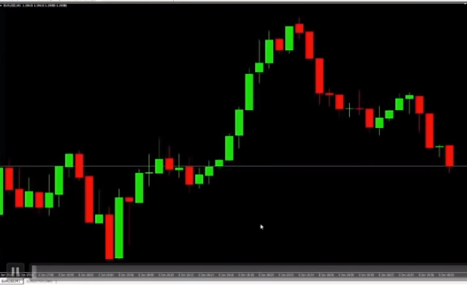
\includegraphics[scale=.65]{images/graphs-03.png}
        \end{tabular}
    \end{center}
    Podemos observar esas mechas que nos indican máximos y mínimos y, teniendo en cuenta los colores, sabemos si el precio de apertura y cierre ha sido uno mayor o menor que el otro. Al final del gráfico vemos como se va construyendo la barra, puede comenzar con un máximo o un mínimo o en ocasiones por la mitad, hasta que no finalice ese período de tiempo no tendremos una \ti{vela cerrada}.
    \item kkk
\end{enumerate}

\section{Teoría de Dow. Líneas de tendencia, soporte y resistencia}

La \tb{Teoría de Dow} fue propuesta por \ti{Charles Henry Dow} (1851-1902), que en el siglo XIX planteó una serie de enunciados relacionados con los movimientos bursátiles; se basó en dos indicadores que el mismo Dow creó:
\begin{itemize}
    \item \ti{Dow Jones industrial average (DJIA)}
    \item \ti{Dow Jones transportation average (DJTA)}
\end{itemize}
los formuló para intentar ponderar de alguna manera los movimientos de la economía real, siendo estos dos sectores muy importantes en el motor de las economías. A partir de estos dos indicadores o índices planteó las diferentes proposiciones o enunciados de lo que ha conformado la \ti{teoría de Dow}:

\begin{enumerate}
    \item Las medias lo descuenta todo, esto implica que la evolución diária de estos dos índices (DJIA y DJTA) recogen toda aquella información y expectativas disponibles de los inversores.
    \item El mercado tiene \ti{tres tendencias}:
    \begin{itemize}
        \item \ti{Tendencia primaria}, a su vez se observan tres fases:
        \begin{itemize}
            \item de acumulación,
            \item expansión y 
            \item agotamiento o distribución.
        \end{itemize}
        Es la base funcamental en la que se basa el análisis técnico, es una tendencía con una duración que va de meses a años, no es exacta pero es aproximada y váldia para inversiones a largo, hasta que se agota dicha tendencia.
        Cómo se plantea una tendencia alcista, en este caso sería la \ti{unión de los mínimos}, que se corresponde con una sucesión de máximos y mínimos crecientes.
        \begin{center}
            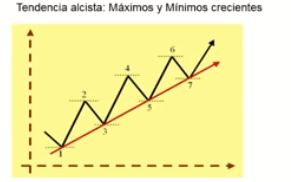
\includegraphics[scale=.80]{images/tendencia-alcista.png}
        \end{center}
        Por el contrario, para identificar una \ti{tendencia bajista} nos fijamos en cotizaciones de precios con máximos y mínimos decrecientes, uniríamos esos máximos con los mínimos y tendríamos la línea de tendencia bajista.
        \begin{center}
            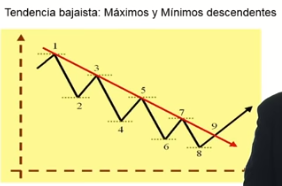
\includegraphics[scale=.80]{images/tendencia-bajista.png}
        \end{center}
        Mientras esas líneas (tendencias) no se rompan la línea sigue siendo vigente.
        \item \ti{Tendencia secundaria}, no son más que oscilaciones dentro de la tendencia primaria, su duración es más corta, entre semanas y meses, y significan o pueden suponer ciertas correcciones, entre $1/3$ y $2/3$ de la tendencia primaria. No es una matemática exacta, no tiene por qué cumplirse siempre, pero estadísticamente, a lo largo del tiempo, suelen corregir este tipo de porcentajes. 
        Operar bajo estas tendencias está dirigida a inversores de medio y corto plazo.
        En el siguiente gráfico vemos una \ti{tendencia primaria creciente}
        \begin{center}
            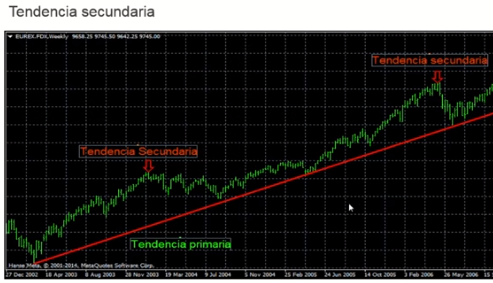
\includegraphics[scale=.80]{images/graphs-01_02.png}
        \end{center}
        observamos los mínimos y máximos crecientes (tendencia primaria) y vemos unas \ti{tendencias secundarias} que se inician en los puntos marcados, donde los precios retroceden.
        \item \ti{Tendencia terciaria}, su duración es muchísimo más corta, inferior a tres semanas. Las fluctuaciones se suceden dentro de las \ti{tendencias secundarias}, Se plantea para inversiones a \ti{corto o muy corto plazo}
        \begin{center}
            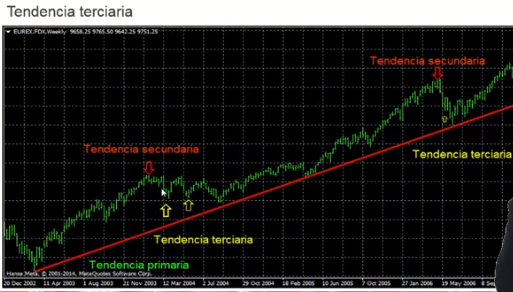
\includegraphics[scale=.80]{images/graphs-01_03.png}
        \end{center}
        observamos en el gráfico, dentro de la tendencia secundaria, las oscilaciones pertenecientes a la \ti{tendencia terciaria}, que requieren un cierto nivel de conocimiento mucho más avanzado.
    \end{itemize}
    \item Tenemos un \ti{principio de confirmación}, donde las señales de compra o de venta (cambios de tendencia) deben confirmarse cuando los índices se comportan en la misma dirección.
    \item El volumen debe acompañar siempre a la tendencia, lo que implica que debe haber o existir un incremento de volumen cuando los precios van en la dirección de la tendencia, si es alcista; cuando la tendencia es bajista, el volúmen debe contraerse.
    \item Las tendencias siempre se mantienen vigentes hasta que se confirme una señal de cambio, para ello aparecen las denominadas líneas de \ti{soporte} y \ti{resistencia}. Estas líneas, según la \ti{teoría de Dow} son las que nos pueden indicar o poner en alerta en momentos en los que los precios se detienen.
    \begin{itemize}
        \item Una línea de soporte sería la zona en la que existe cierta concentración de demanda, lo que implica que los precios vienen bajando hasta que llega un momento que se detienen, y esto sucede porque existe un incremento de la demanda respecto de la oferta.
        \item Una línea de resistencia sería lo contrario, los precios van subiendo hasta que llega un momento que se detienen y esto se produce porque se incrementa la oferta de títulos.
    \end{itemize}
    Cuando estas líneas se rompen, cambian su papel, si antes era una línea de soporte, y se rompe, cuando los precios vuelvan hacia ella se combierte en una línea de resistencia, y al contrario con las líneas de resistencia.
    \begin{center}
            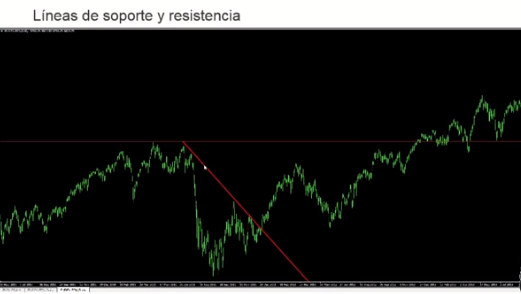
\includegraphics[scale=.80]{images/soporte_resistencia.png}
        \end{center}
    En el gráfico vemos que los precios han ido subiendo, llegado un punto parecen que se detienen, en ese punto podemos dibujar una línea horizontal a lo largo del gráfico que se corresponde con la \ti{línea de soporte}, los precios oscilan, subiendo y bajando, pero no llegan a romper esa línea. Observamos que los precios comienzan a bajar y hay una zona bajista donde los precios caen con fuerza hasta que llega un momento en que se detiene, en ese momento se observa un incremento de la demanda de títulos, de nuevo podemos dibujar, en este caso una \ti{línea de soporte}, mientras los precios rebotan arriba y abajo, y se observa una posible líne alcista a partir de la \ti{línea de soporte}, ésta unirá los mínimos en una \ti{línea de tendencia primaria}. Se observa que los precios van rebotando en es línea de tendencia alcista, y se observa como llega un punto en el que se rompe la \ti{línea de resistencia}, observándose una zona de \ti{falsa rotura}, donde no es claro que siga la tendencia, pero de nuevo rompe la línea de soporte, caen los precios para a continuación volver a romper la línea de soporte y seguir con la tendencia alcista.
\end{enumerate}

Todos estos principios se plantean para una versión más a medio y corto plazo, aunque es posible aplicarlas a largo plazo. La diferencia fundamental es que este tipo de análisis técnico es más útil para aquellas gestiones más activas del inversor, que compra y vende títulos con cierta frecuencia, frente a la inversión pasiva, donde el inversor hace una compra y mantiene la posición quince o veinte años.

\section{Medias móviles}

Las \ti{medias móviles} son una serie de herramientas para identificar \ti{tenencias} y \ti{cambios de tendencia}.

¿Qué es una media? La \ti{media} estadísticamente la suma de un conjunto de datos dividido por el número de elementos. 

El concepto de \ti{media móvil} implica que vamos a recalcular dicha media eliminando el último dato e incorporando un nuevo dato. Estos datos que se incorporan pueden ser muy variados, lo más habitual es utilizar los precios de cierre; se pueden utilizar el máximo y el mínimo de cada barra de vela o incluso valores del propio indicador.

Otra característica de las medias, es que el número de elementos puede ser variable, podemos determinar el período de retardo o de datos anteriores que vamos a utilizar para calcular dicha media:
\begin{itemize}
    \item un número pequeño \tb{implica} que obtendremos una \ti{media móvil más corta}.
    \item un número más alto \tb{implica} una \ti{media móvel más larga}.
\end{itemize} 

En análisis técnico existen tres tipos básicos de \ti{medias móviles}:

\begin{itemize}
    \item \tb{media móvil simple (SMA)}: es el cálculo de los períodos, en este caso de los cierres de los últimos 10 períodos
    $$
    \mathit{SMA} = \frac{C_{10} + C_{9} + C_{8} + \ldots + C_{2} + C_{1}}{10}
    $$
    \begin{center}
        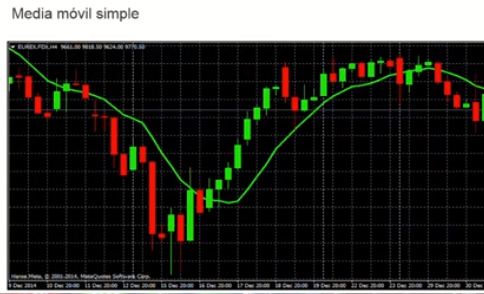
\includegraphics[scale=.80]{images/medmovsim.png}
    \end{center}
    En el gráfico podemos ver que la media móvil simple no es más que un alisado de los precios bursátiles, en función del número de períodos que cojamos nos aproximaremos más a los precios, o por contra se desplazará más hacia la derecha, la media.
    \item \tb{media móvil ponderada (WMA)}. Lo que se hacemos es una \ti{ponderación} dando unos pesos específicos a cada uno de sus precios de cierre. En este caso se le da siempre más importancia a aquellos cierres más cercanos al actual.
    $$
    \mathit{WMA} = \frac{1\ast C_{10} + 2\ast C_{9} + 3\ast C_{8} + \ldots + 9\ast C_{2} + 10\ast C_{1}}{10+9+8+7+6+5+4+3+2+1}
    $$
    Haciendo una comparativa entre \ti{SMA} y la nueva \ti{WMA} tenemos el siguiente gráfico:
    \begin{center}
        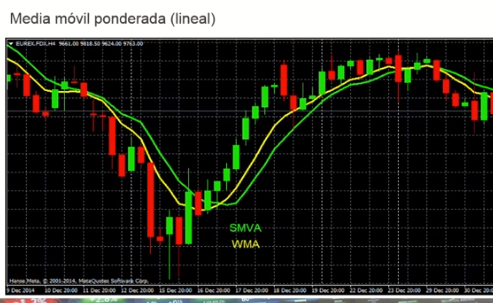
\includegraphics[scale=.80]{images/medmovpon.png}
    \end{center}
    vemos cierto desplazamiento de una u otra.
    \item \tb{media móvil exponencial (EMA)}. Su cálculo es un poco más complejo, sin embargo, estos cálculos no es necesarios hacerlos manualmente, hoy en día todas las plataformas de traiding tienen incorporado este tipo de formulación, lo único que tendremos que indicar es los precios o el valor que queremos incorporar a ese cálculo, es decir, sólo los precios de cierre o los máximos o los mínimos, y el período de tiempo que queremos utilizar.
    \begin{center}
        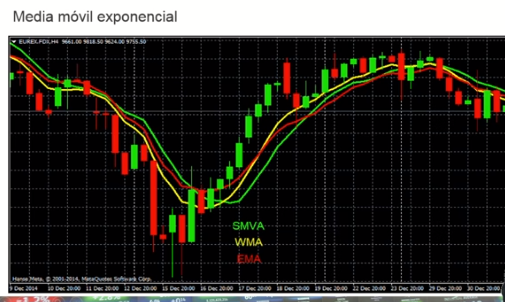
\includegraphics[scale=.80]{images/medmovexp.png}
    \end{center}
    La media exponencia viene indicada por la línea rojas, vemos un movimiento de alisado, en cuanto a la elección de una u otra medida, va un poco en función de la forma de operar de cada trader. 
\end{itemize}

Existen múltiples estrategias, que utilizarán alguna de las medias vistas, si bien la utilización individual de una de ellas no aporta especial relevancia, en cambio la combinación o cruce entre dos o más medias si es relevante.

En cuanto al plazo a seleccionar, aquellos más cortos estarán más próximos al precio, por lo que puede haber más cruces con dicha media, mientras que plazos más largos implican más desplazamiento hacia la derecha y cruces menos habituales.

¿Cómo identificar una tendencia con la \ti{media móvil}? Simplemente con el cruce respecto del precio de cotización.
\begin{center}
    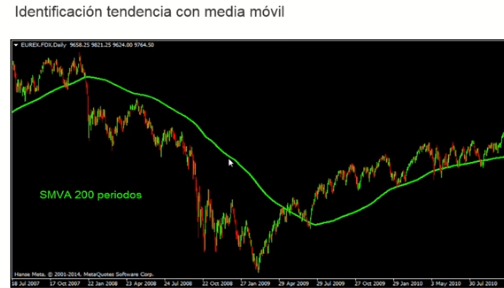
\includegraphics[scale=.80]{images/identificar-tendencia.png}
\end{center}
en este caso tenemos una media simple  de 200 períodos, muy habitual para identificar tendencias a largo plazo, donde efectivamente observamos como cuando los precios rompen a la baja, la media móvil comienza una tendencia bajista. Además, en este caso hablamos de precios diarios y es bastante larga. 

¿Qué ocurre cuando esos precios rompen al alza la línea media móvil? Da comienzo a una \ti{línea de tendencia alcista}, por lo que las medias móviles pueden sernos útiles para identificar cambios de tendencia.

Es importante tener en cuenta que los \ti{cruces de medias móviles} no siempre son rentables en el \ti{largo plazo}, pero sí que pueden ser muy identificativos de posibles cambios de tendencia.

\section{MACD}

El \tb{MACD} es un \ti{indicador técnico}, éstos son herramientas dentro del análisis técnico, cuyos objetivos se concretan en: 
\begin{itemize}
    \item análisis cuantitativo, que recogen una serie de indicadores y osciladores que pueden albergar diferentes tipos de objetivos. 
    \item identificar anticipadamente cambios de tendencia. Como vimos, ésto vendría motivado porque las \ti{líneas de tendencia primaria}, unión de diferentes puntos mínimos o máximos, hasta que no empieza el movimiento o ha transcurrido un cierto tiempo de ese movimiento, no podemos identificar si es una línea de tendencia \ti{alcista} o \ti{bajista}, con los indicadores técnicos pretendemos anticipar ese cambio de tendencía.
    \item determinar la fortaleza de la tendencia, si la tendencia que se ha iniciado tiene la suficiente fuerza compradora, en el caso de tendencia alcista, o si se trata de una tendencia bajista, tiene fuerza suficiente para mantenerla.
    \item indicar o facilitar señales de compra o venta para realizar nuestro trading.
    \item identificar situaciones de sobrecompra o sobreventa, zonas en las que hay demasiados compradores, que saturan el mercado, y puede haber cambios de tendencia o sobreventa en los que los precios han bajado tanto que hay exceso de venta de títulos, y es posible que se pueda esperar un cambio de tendencia.
    \item pueden utilizarse como identificadores de \ti{divergencias entre los precios de las cotizaciones} y el \ti{indicador}. Si los precios de cotización van en una dirección alcista y los indicadores permiten trazar una línea bajista, existe una divergencia entre ambos que nos indicaría un posible cambio de tendencia. Y al contrario, si los precios están bajando y el indicador prevee una línea alcista, también implicaría un cambio de tendencia.
\end{itemize}

Uno de los indicadores más habituales en todas las plataformas de trading sería el \ti{Moving Average Convergence Divergence (MACD)}, se compone básicamente de dos  líneas, sus fórmulas no son necesario calcularlas manualmente ya que las propias plataformas facilitan dichos cálculos:

\begin{enumerate}
    \item Diferencia entre dos \ti{medias exponenciales}, una corta y otra larga, en función de los períodos, los más habituales son 26 y 12 años, aunque el usuario puede modificarlos.
    $$\mathit{MACD} = \mathit{EMA}(C,26) - EMA(C,12)$$
    \item Define la \tb{lína de señal} , que se calcula como la \ti{media exponencial} de 9 períodos sobre el \ti{MACD}, que habíamos calculado, y como el anterior, puede ser modificado por el usuario:
    $$\text{SEÑAL} = \mathit{EMA}(\mathit{MACD},9) $$
\end{enumerate}

Las señales se genera cuando la \ti{línea de señal} cruz a la \ti{media del MACD}, bien hacia arriba, señales de compra, o hacia abajo, señales de venta.

\begin{center}
    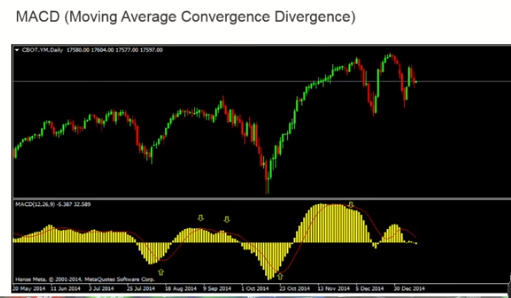
\includegraphics[scale=.80]{images/MACD.png}
\end{center}

Vemos en el ejemplo diferentes tipos de señales. En la parte inferior vemos un cruce de la línea de la señal, línea roja, con los precios de la señal \ti{MACD}, generaría una señal de compra. A continuación vemos otro cruce, que en este caso sería una señal a la baja, de venta.

A veces puden ocurrir diferetnes tipos de señales intermedias, siendo la forma más habitual el \ti{filtrar} y sólo hacer caso de aquellas señales de compra o cruces que se generan por debajo de la \tb{línea cero}, y las de venta sólo aquellas que estén en la parte superior de dicha línea.

A continuación mostramos gráficos con diferentes ejemplos de señales:

\begin{center}
    \begin{tabular}{ c }
        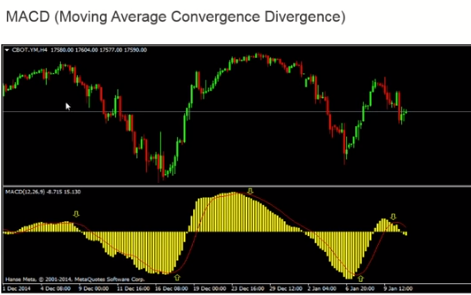
\includegraphics[scale=.80]{images/MACD-01.png} \\
        \\
        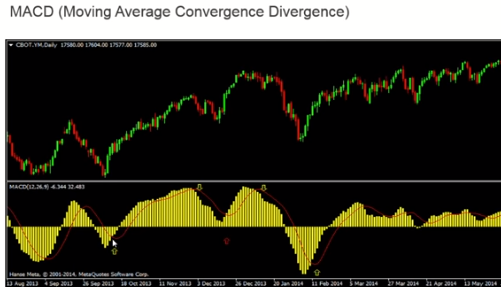
\includegraphics[scale=.80]{images/MACD-02.png}
        
    \end{tabular}
\end{center}

En el segundo gráfico observamos una señal de compra hacia la mitad del gráfico, que consideramos arriesgada pues se encuentra por encima de la \ti{línea de cero}, y hemos dicho que deberíamos hacer caso de aquellas que están por debajo de cero, y las ventas por encima de dicha línea, lo ideal sería filtrarlo como indicamos anteriormente.

\section{Time frame y fractalidad}

Podemos hacer una definición de \tb{fractal} partiendo de la idea del matemático \ti{Mandelbrot (1975)} que definió \ti{fractal} como \ti{«una figura, que puede ser espacial o plana, formada por componentes infinitos»}. Eto implica que tiene una característica pecualiar, que es que la apariencia, la forma como se distribuye, estdísticamente es similar, con independencia de qué escala de observación tengamos sobre la figura. Si hacemos zoom sobre la figura veremos, que la estructura, se repite a lo largo de los distintos zoom que realicemos. El gráfico es una imagen intuitiva en la que vemos como se repiten estos picos:
\begin{center}
    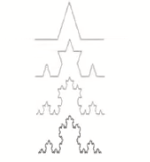
\includegraphics[scale=.80]{images/fractal.png}
\end{center}

El \tb{time frame} consiste en como se representan los precios de cotización, vimos que gráficamente se representan mediante gráficos de líneas, barras y velas, y cada una refleja cierta información en un período de tiempo concreto.

Los elementos que lo componen están referenciados a un período de tiempo concreto.

El siguiente es un ejemplo de \ti{time frame} mediante un gráfico de barras en el que observamos como para un \ti{time frame}, en este caso, cada barra representa la información sucedida durante cada una de esas horas:

\begin{center}
    \begin{tabular}{ c }
        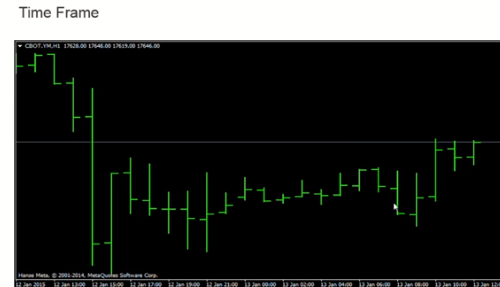
\includegraphics[scale=.80]{images/time-frame.png}
        \\
        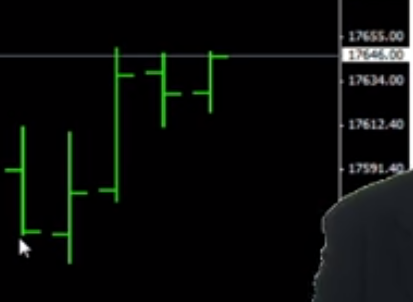
\includegraphics[scale=.80]{images/time-frame-01.png}
    \end{tabular}
\end{center}
En el segundo gráfico, la barra más a la izquierda, representa con la rayita de la izquierda representa la apertura con el primer precio cotizado en esa hora, y la inferior de la derecha, el precio de cierre en esa hora, el máximo y el mínimo, fin superior e inferior de la barra, repesentan el máximo y mínimo alcanzado entro de esa hora, y así sucesivamente.

¿Cómo se unen la fractalidad y el time frame con el análsis técnico?
\begin{center}
    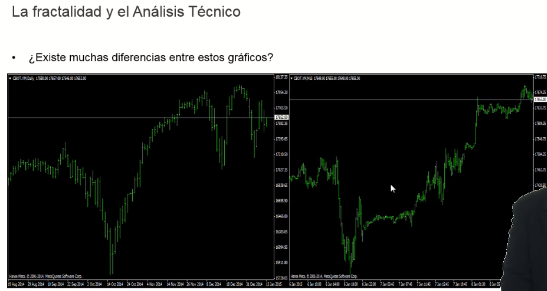
\includegraphics[scale=.80]{images/time-frame-02.png}
\end{center}

Respondiendo a la pregunta que se muestra en la imagen, a priori podemos observa que hay movimientos que van hacia abajo y hacia arriba, tendencias alcistas y bajistas, en ambos gráficos. Ambos gráficos representa un mismo tipo de activo, el índice Dow Jones. El gráfico de la izquierda representa un \ti{time frame diario}, el de la derecha es un \ti{time frame quince minutos}. Esto nos permite pensar que la utilización de la fractalidad nos permite usar todas las herramientas de \ti{análisis técnico lateral de Dow} sobre los \ti{time frame de los activos}, lo único es que hay que adaptarlo a cada uno de ellos. Puede ser que haya indicadores que funcionan bien en time frame largos, en aquellos más cortos deban ajustarse, pero la base fundamental de las líneas de tendencia soporte,  resistencia, etc de la teoría de Dow es plenamente factible en cualquier time frame.

Por ejemplo, en el siguiente gráfico, representación de un time frame de una hora, observamos una línea de tendencia alcista que parte de la parte inferior de la gráfica:

\begin{center}
    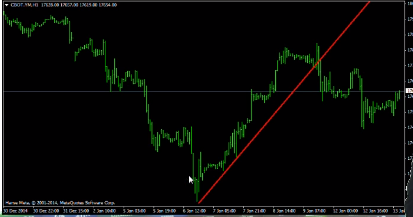
\includegraphics[scale=.80]{images/time-frame-03.png}
\end{center}

En el siguiente, tenemos un time frame de quince minutos y tenemos una línea de tendencia bajista.

\begin{center}
    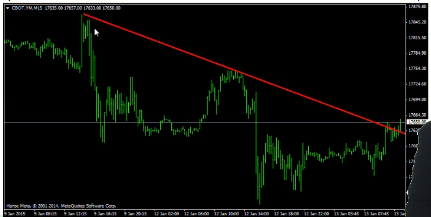
\includegraphics[scale=.80]{images/time-frame-04.png}
\end{center}

con lo que vemos que es posible la utilización de estas herramientas en el análisis técnico.


